\chapter{Hello World}
Python is a programming language, developed by the Python Software Foundation and released under the PSFL License. I quote Wikipedia: \begin{quotation}
`Python is an interpreted, high-level, general-purpose programming language. Created by Guido van Rossum and first released in 1991, Python's design philosophy emphasizes code readability with its notable use of significant white space. Its language constructs and object-oriented approach aim to help programmers write clear, logical code for small and large-scale projects.
\end{quotation}
For those who have never programmed in their lives, Python offers an easy in of sorts, as the language is very easy to both read and use.
\section{Python installed?}
To check if you have Python already installed, open the command prompt and type \begin{quote}
Python
\end{quote}
If Python is installed, the command prompt should reply
\begin{quote}
Python 3.8.3 (tags/v3.8.3:6f8c832, May 13 2020, 22:37:02) [MSC v.1924 64 bit (AMD64)] on win32\\
Type "help", "copyright", "credits" or "license" for more information.\\
$>>>$
\end{quote}
However, if you don't see a message like above, but instead see:
\begin{quote}
'python' is not recognized as an internal or external command,\\
operable program or batch file.
\end{quote}
then, you don't have a copy of Python on your computer.
To install Python, go to www.python.org/downloads/ and follow the instructions\\
Now that all of us have Python installed on our computers, we may begin or exploration of the language.
\section{First program}
Finally, our first program. Our aim is to print the statement "Hello World" (Interestingly, the tradition began with Ritchie \& Kerningham's book `The C Programming Language')\begin{quote}
print("Hello World!")
\end{quote}
Would simply return:
\begin{quote}
Hello World!
\end{quote}
In Python 3, the statement \emph{print()} was used to print a statement, which in the above case was a string which was enclosed in "double quotes". 
\section{More Printing}
If we so desire, we may also print multiple strings at the same time using the \emph{print()} function as shown:
\begin{quote}
print("Hello World!","Hoorah!!")
\end{quote}
which would return
\begin{quote}
Hello World! Hoorah!!
\end{quote}
The \emph{print()} function inserts a newline after printing the arguments passed to it. So in other words,
\begin{quote}
print("Hello World!","Hoorah!!")
\end{quote}
and 
\begin{quote}
print("Hello World!")\\
print("Hoorah!!")
\end{quote}
Would return two different outputs as shown
\begin{quote}
Hello World! Hoorah!!
\end{quote}
and 
\begin{quote}
Hello World!\\
Hoorah!!
\end{quote}
respectively.\\
To force the printing of a newline, we use "\textbackslash n" in our string as shown.
\begin{quote}
print("Hello World! \textbackslash n Hoorah!!")
\end{quote}
The above script returns the same output as:
\begin{quote}
print("Hello World!")\\
print("Hoorah!!")
\end{quote}
But the former is preferred for the sake of brevity.\\
In a similar manner, we may also format output with "\textbackslash t" to force a new tab, and "\textbackslash r" to force the cursor to return to the start of the line.\\
It is useful to know that "\textbackslash" character is also called an "Escape Character", that converts a special(reserved) symbol into an ordinary character.
\section{Variable Variables}
Now that we have started using the \emph{print()} function, we may further explore it.\\
the print function can also print the value of variables.
\begin{quote}
somevariable="Hello World, I am a variable"\\
print(somevariable)
\end{quote}
returns
\begin{quote}
Hello World, I am a variable
\end{quote}
The variable can the be reset to another value if needed.\\ In short, a single 'equals' mark indicates assignment of a variable.
The entire process can be described as: 
\begin{figure}[hbt]
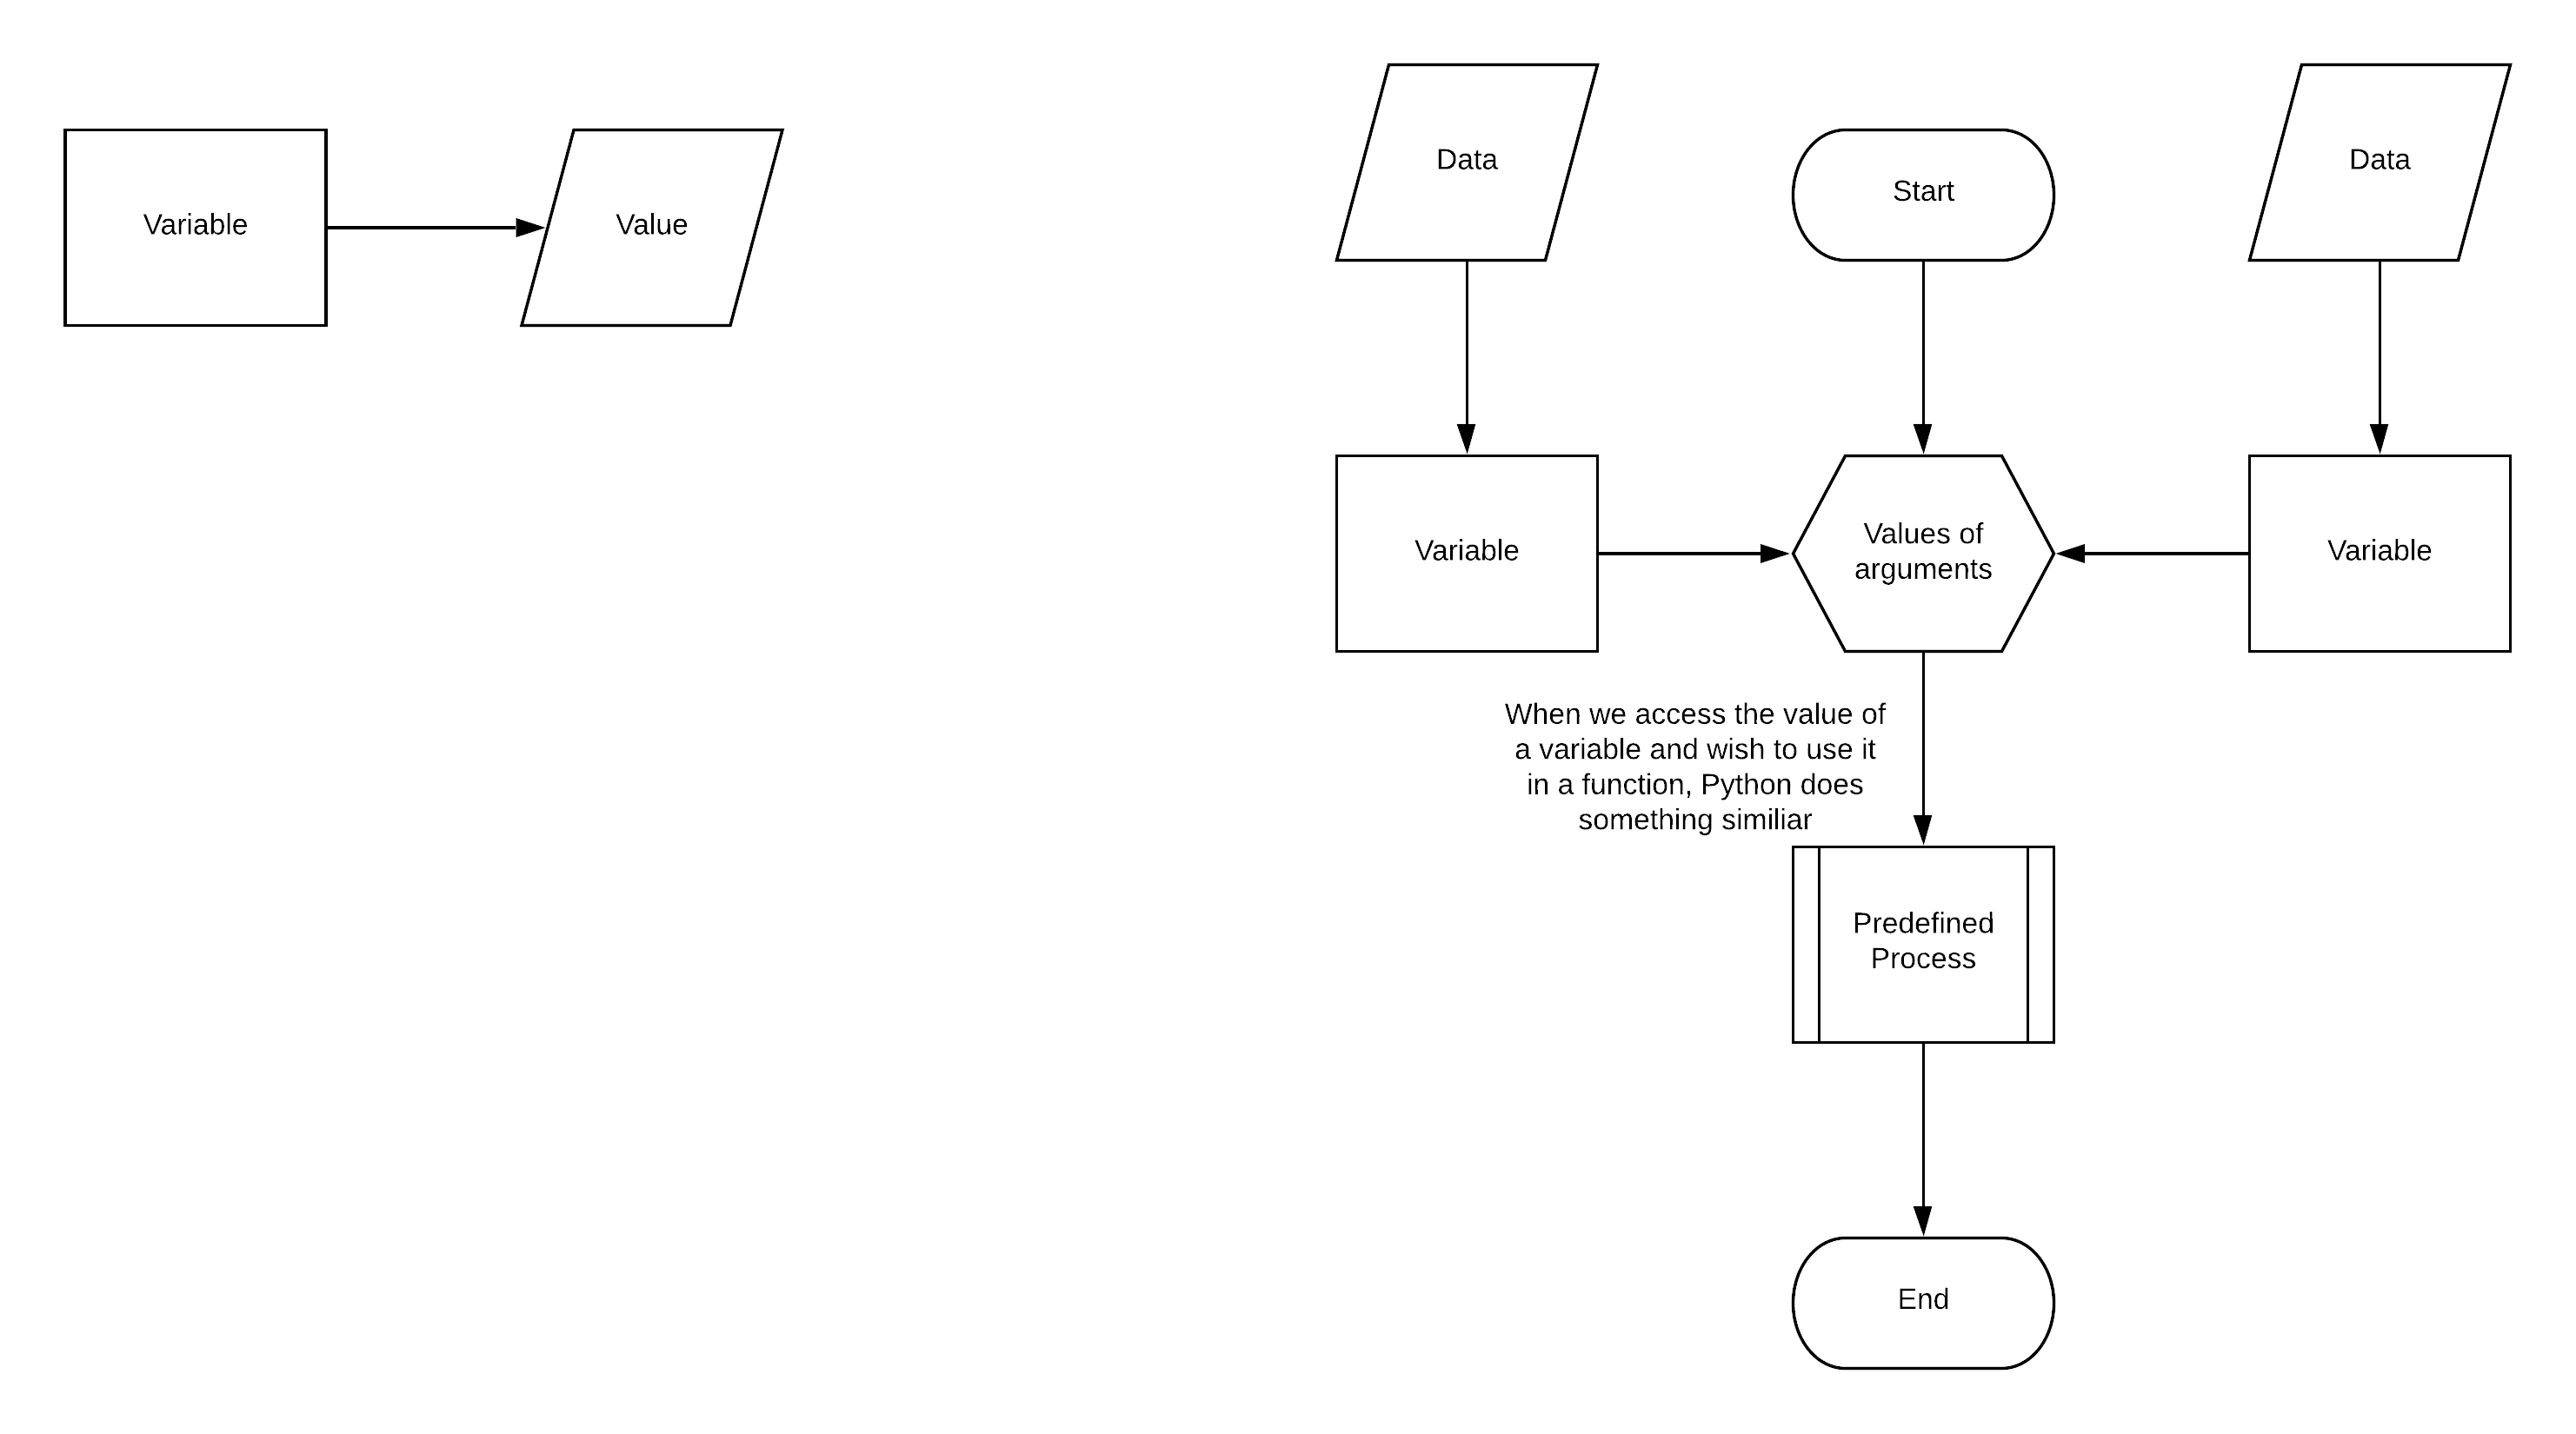
\includegraphics[scale=0.25]{flowchart}
\end{figure}
\\
In Python, all variables are not \emph{declared}, they are \emph{assigned}. This highlights the fact that Python is Dynamically typed.\\ Dynamically typed means that the type of a variable is checked during run-time, and not during \emph{declaration}. \\ \\ 
NB: A language is statically-typed if the type of a variable is known at compile-time instead of at run-time. A more comprehensive list of differences can be found in Appendix A
\\ \\

We may also print multiple variables and/or strings at the same time, as with strings, in a similar fashion. For example:
\begin{quote}
var1="abc"\\
var2="def"\\
print(var1,var2,"ghi")
\end{quote}

Which would return:
\begin{quote}
abc def ghi
\end{quote}

\section{Basic Operations}
Python, like most programming languages has some basic math in it's Standard Library. The four operators viz. `+' `-' `*' and `/' are used with both variables an constants alike.
\\ \\ NB: A more comprehensive list of mathematical functions(among others) can be found at the end of the book in Appendix B\\ \\
 For example to find and print the product of 256 and 456, we can use:
\begin{quote}
a=256\\b=456\\c=a*b\\print(c)
\end{quote}
The shell would return:
\begin{quote}
    116736
\end{quote}
As explained before, the  \emph{print()} function takes both variables and strings as inputs concatenates the values of both in place.This allows us to easily `dot the i's and cross the t's '. For example, to calculate the value of $234/2$ and print it's value, the following script can be used:

\begin{quote}
num=234\\
dividend=2\\
print("The quotient of",num,"and",dividend,"is",num/dividend)
\end{quote}
would return:
\begin{quote}
117.0
\end{quote}

In the above script, we used \emph{num/dividend}, 
Note that the shell returns 117.0 and not 117. In Python, the presence of a decimal is indicative of the number being a /emph{floating point} number(It will be covered later on). In short, it cannot be compared to an integer (A number without a decimal point).

\newpage	
\section{Exercises}
\begin{enumerate}
\item Write a program to convert \emph{Celsius} to\emph{Fahrenheit} for the given temperatures $t=45^{\circ}$C and $t=-40^{\circ}$C.
\item Write a program that calculates the average of three numbers 189086, 127809, 1567801.
\end{enumerate}



